\subsection{Target Areas in the Gulf of California and Dataset Statistical Analysis}
\begin{figure}[t]
    \center
    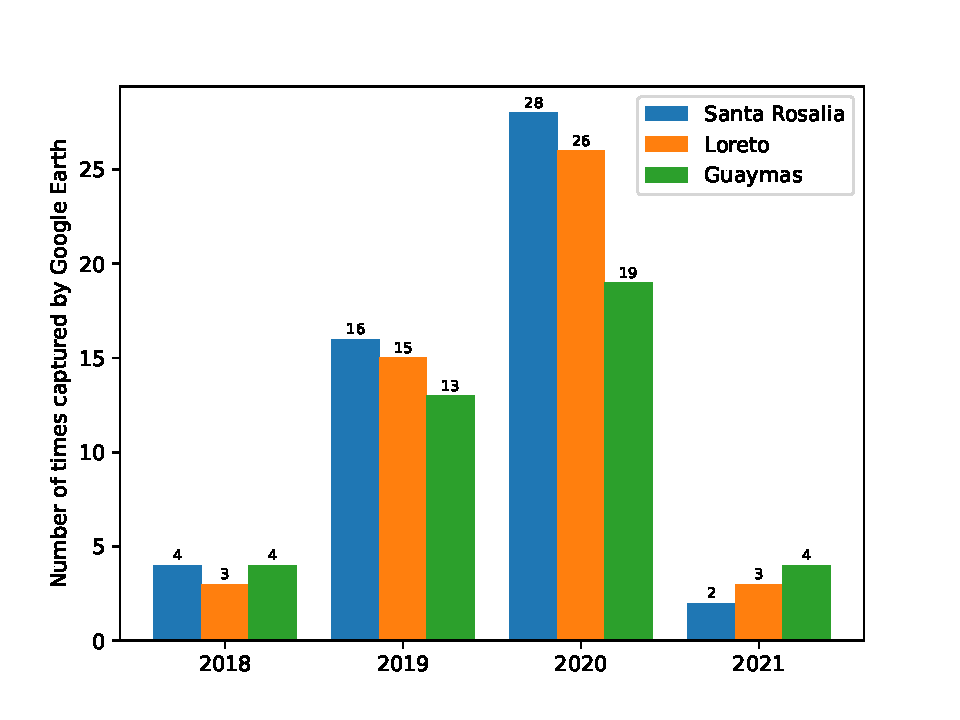
\includegraphics[width=\columnwidth]{img/NumberOfTimesCapturedByGEP.pdf}
    \caption{Number of times the three cities (Santa Rosalia, Loreto, Guaymas) captured by Google Earth Pro from 2018 to 2021.}
    \label{NumberOfTimesCapturedByGEP}
\end{figure}

The Gulf of California in Mexico was chosen as an area of study. Ideally, to analyze a sufficient amount of satellite image data, the ports of each of the major harbor cities in the Gulf of California would need to be included in the scope of our study. Thus, the first step in the work was to find out if there was enough satellite data for the area. In this study, we separate the Gulf of California into few parts on the Mexican state limits: (1) Baja California, (2) Sinaloa, (3) Sonora, (4) Baja California Sur. The satellite dataset used in this analysis includes 694 high-resolution images of ships around the world collected from Google Earth~\cite{lutherborrowship}. From the imagery dataset it was performed an statistical analysis on how many times, temporally speaking, the satellite database captured the region of interest. As a result of this analysis it was found out that:
\begin{itemize}
    \item most cities in the Gulf of California do not have enough satellite data in 2018 and in 2021 while many cities have relative rich satellite data between 2019 and 2020;
    \item there is a steady increase in the collection of satellite data in the Gulf of California from 2018 to 2020;
    \item the open-access and high-quality satellite data from Google Earth Pro is not immediately available for the public;
    \item differences in data accessibility are still evident among different cities. For example, it is accessible for some cities, like Guaymas in the state of Sonora, to have rich satellite images in 2019 and in 2020. However, some cities, such as La Ventana in the state of Baja California Sur, did not appear in Google Earth Pro in 2019 and 2020.
\end{itemize}

\begin{figure}[!t]
    \center
    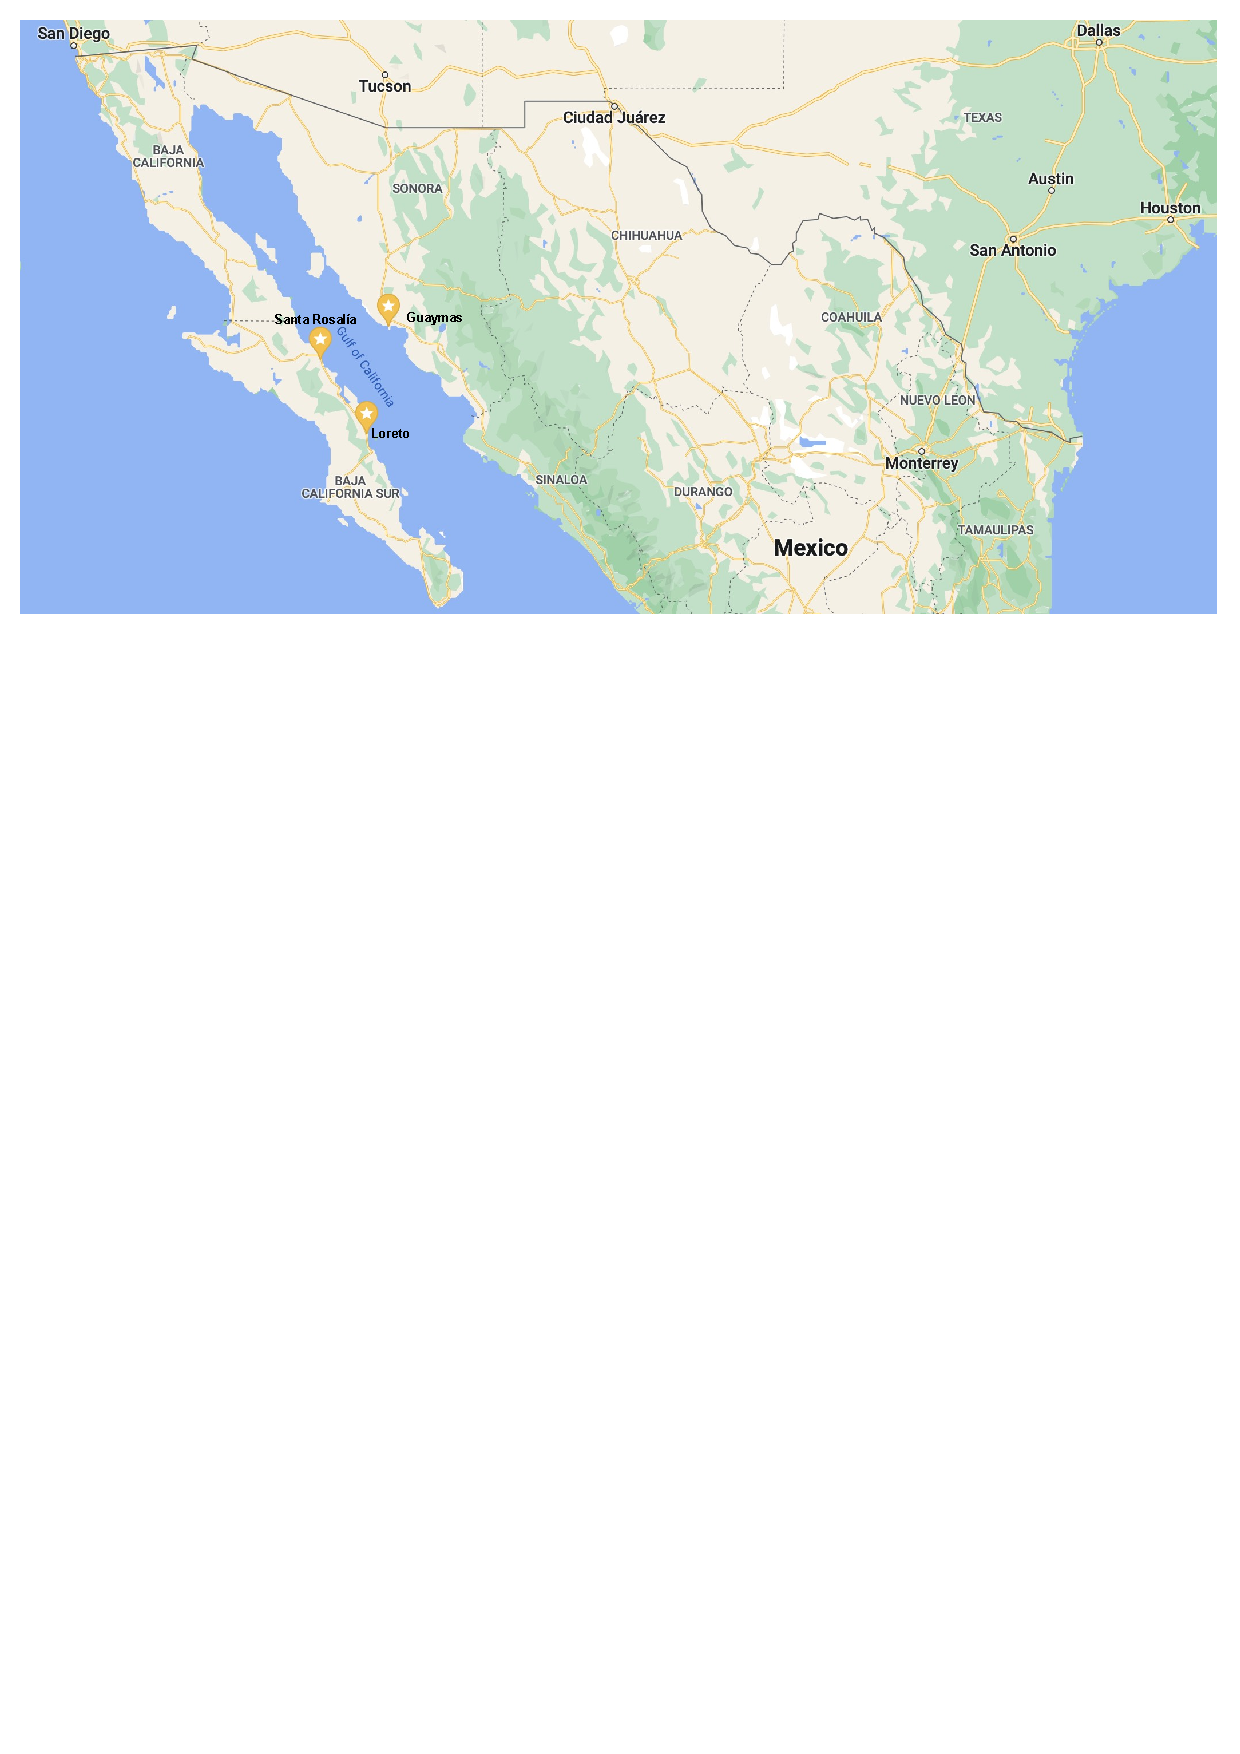
\includegraphics[width=\columnwidth]{img/locations_maps.pdf}
    \caption{The relative geographic locations of the three target cities - Santa Rosalia, Loreto, Guaymas - in Google Maps.}
    \label{locations_maps}
\end{figure}


For this reason, continuing with the previous strategy of analyzing the satellite data for each city in the Gulf of California would lead to a relatively large information bias and thus would not achieve an accurate result of the composition of the boats of the Gulf of California. Therefore, the following three cities with the richest data-accessibility in Google Earth Pro were chosen as the target areas for this study: Santa Rosalia, Loreto, Guaymas, of which the number of times captured by Google Earth Pro~\cite{lisle2006google} is shown in Figure~\ref{NumberOfTimesCapturedByGEP}. Relative geographic locations of the three target cities are shown in Figure~\ref{locations_maps}. The resulting database of the three Mexican coastal cities consisted of 583 images with timestamps between 2019 and 2020.


\subsection{Preprocessing}
Each satellite image was pre-labelled with a highly-precise label box manually~\cite{lutherborrowship}. The original dataset is contained images larger than 9 MB, which is an efficiency burden for the neural network training, especially when there are few objects to be detected. For this reason all the images were resized from 4800 pixels x 2908 pixels to 416 pixels x 416 pixels whose size is approximately 10 KB to 40 KB. 


\subsection{Single Object Detection Architecture}
\label{III-D-Detection-Architecture}

\begin{figure}[t]
    \center
    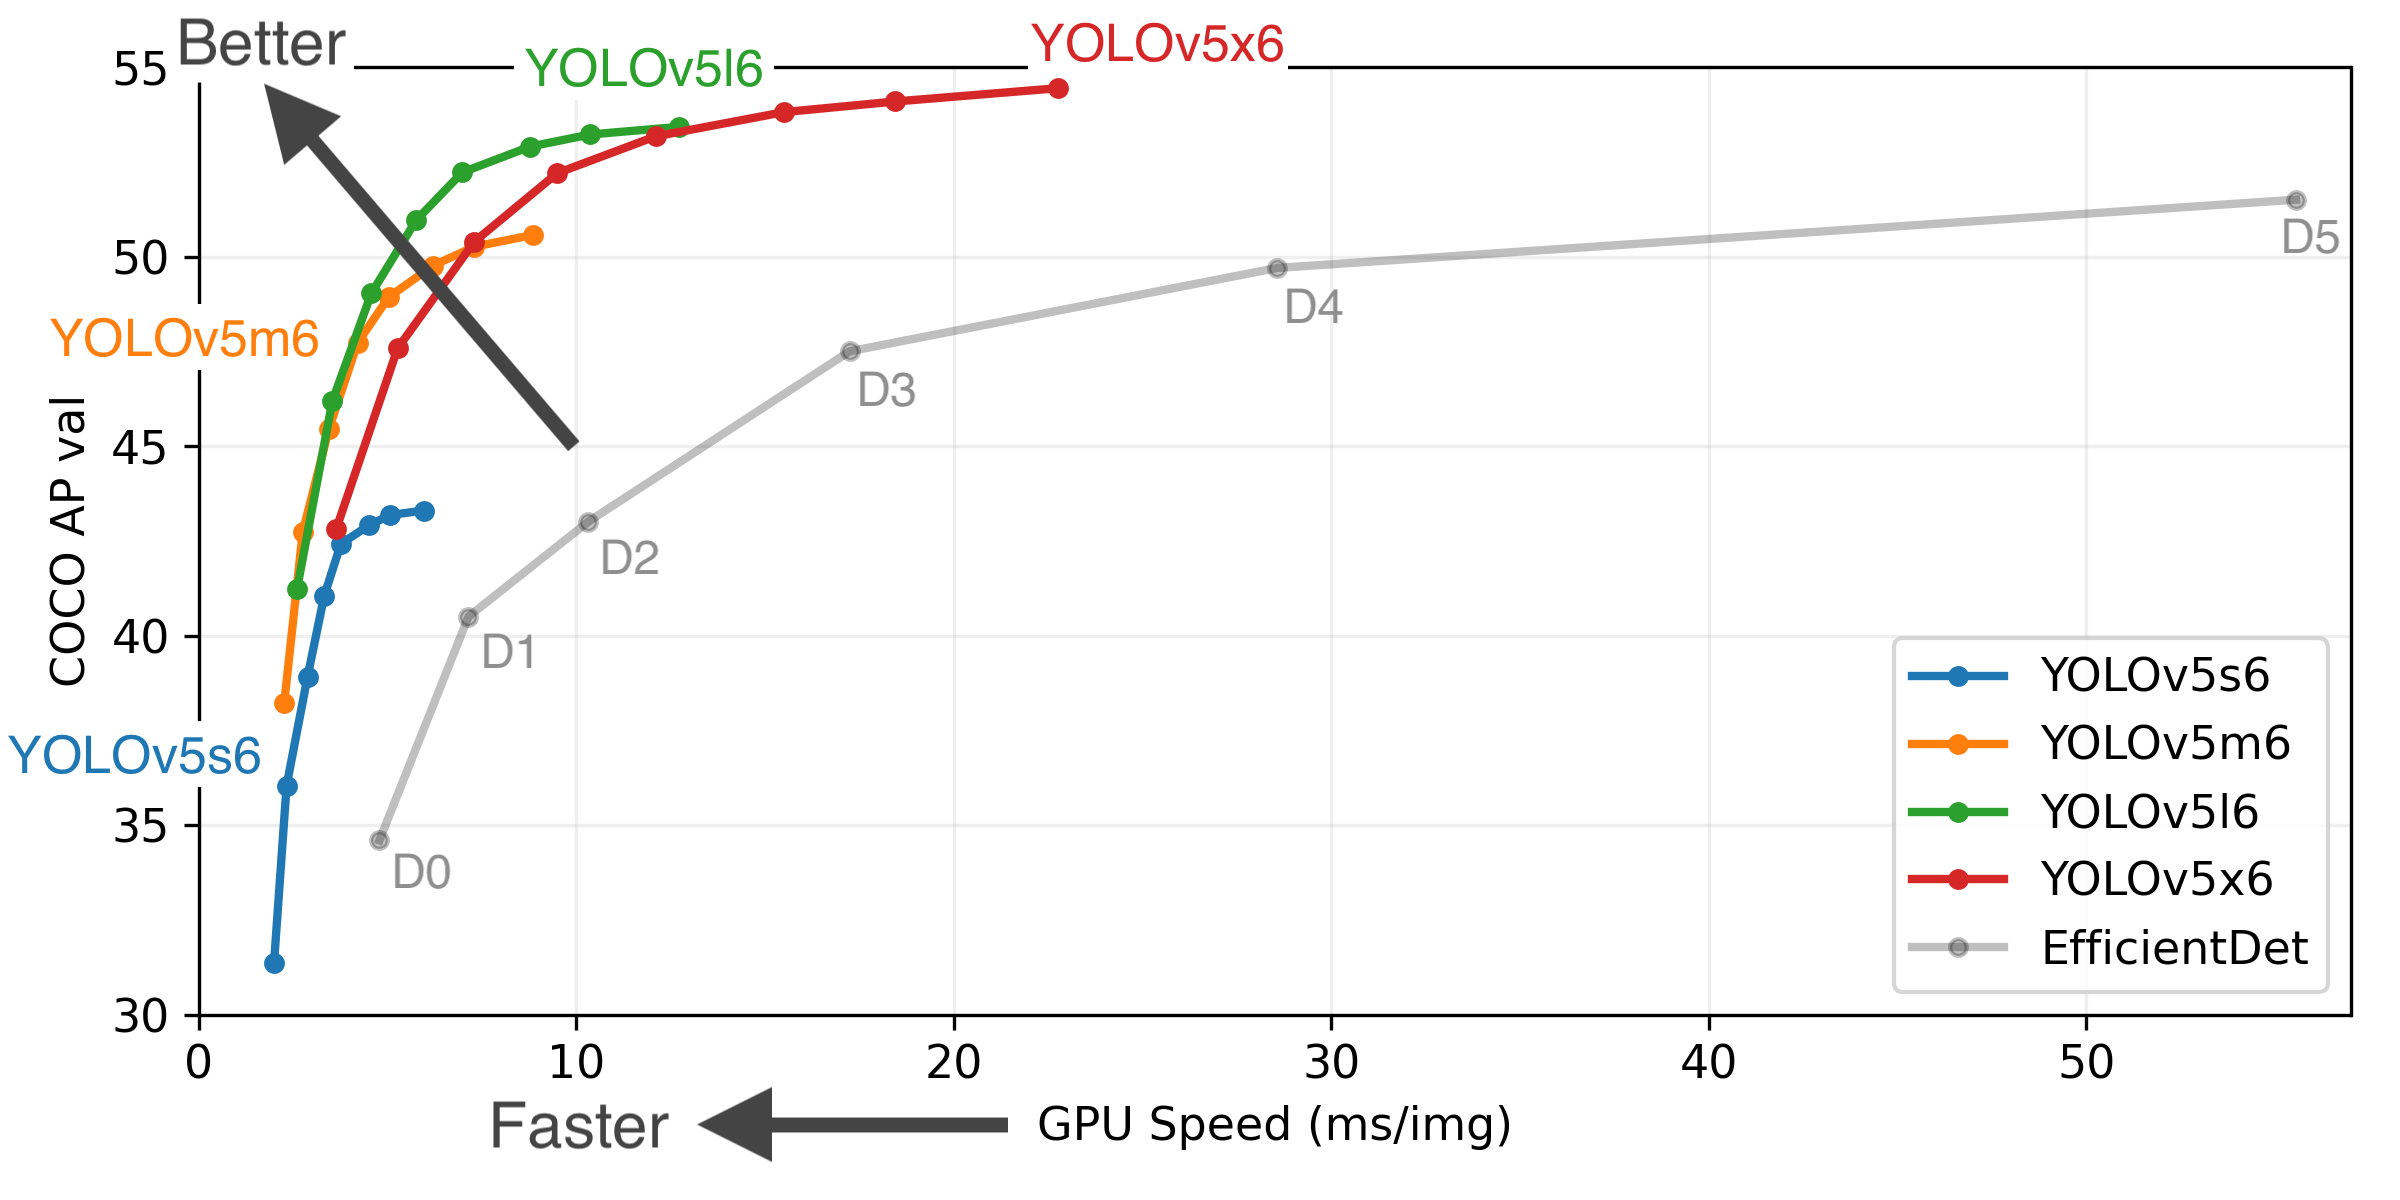
\includegraphics[width=\columnwidth]{img/YOLOv5_Performance.png}
    \caption{{Average Precision (AP) vs. GPU Speed in the 6th generation of YOLOv5 model under COCO data set~\cite{glenn_jocher_2020_4154370}.}}
    \label{fig:YOLOv5_Performance}
\end{figure}

\begin{figure*}[!t]
    \centering
    \includegraphics[width=7in]{img/model_architecture.pdf}
    \caption{\textbf{Model architecture.} Detection model architecture for obtaining a conclusion from an input satellite image of boats.  Images are preprocessed and passed through a CNN. The output of the model is a score, $y \in (0,1)$, representing the probability of being detected as a boat.}
    \label{model_architecture}
\end{figure*}


In Sec~\ref{sec2.2}, recent literature and development of Convolutional Neural Networks (CNNs), including the YOLO model, were discussed. YOLOv5 has four different categories of models, YOLOv5s, YOLOv5m, YOLOv5l, and YOLOv5x~\cite{glenn_jocher_2022_6222936}. They have 7.3 million, 21.4 million, 47.0 million and 87.7 million parameters, respectively. The performance charts can be seen as Figure~\ref{fig:YOLOv5_Performance} where the YOLOv5l model is able to achieve higher average precision with the same faster computing speed. Thus, in this study, the YOLOv5l model was chosen as the model for the training dataset. Figure~\ref{model_architecture} shows a schematic of the models being used for detecting boats, where satellite images in the Gulf of California are as the input of a pre-trained convolutional neural network (CNN). The detection accuracy was determined by computing the the mean probability score from the gulf's satellite images.

Satellite images often have noises, such as shadows cast by water on the sea surface due to sunlight or clouds in the atmosphere. These noises can make the training data inaccurate and often cause problems for the correctness of the model. He et al.~\cite{He2009SingleIH} proposed a simple but effective image prior-dark channel before removing haze from a single input image. The dark channel prior can be used as a statistics of outdoor haze-free images. Based on critical observation, most local patches in outdoor haze-free images contain some pixels whose intensity is very low in at least one color channel. Using this prior-dark channel before the haze imaging model, the thickness of the haze can be estimated, and a high-quality haze-free image can be recovered. Moreover, a high-quality depth map can also be obtained as a byproduct of haze removal.

Similar to the principle of using convolution kernels, specific image kernels can sharpen the image. While the sharpening kernel does not produce a higher resolution image, it emphasizes the differences in adjacent pixel values, making the image look more vivid. Overall, sharpening an image can significantly improve the recognition accuracy of an image with a 5x5 image kernel.

\subsection{Object Measurement and Classification}
Measuring the length of a ship is one of the most challenging topics in this study. As Google Earth Pro does not provide an application programming interface (API) for accurate scales, manually measuring the size of a particular scale became the core of measuring the size of a ship. In this work, all the captured satellite images were set with a fixed eye altitude. By measuring only one real length of the object through Google Earth measurement tool and knowing the pixel length of this object, the length of one pixel in the world of the fixed eye altitude can be calculated.

As the dataset for the training model was created with each edge tangent to the edge of the detected object, it can roughly treat the boat's length as the length of the diagonal of the detection box. Secondly, since the scale is central to the detection of the small boat fleet, the imagery scale should follow the following rules:
\begin{itemize}
    \item cannot be too large. The image needs to contain the full area where boats may be found.
    \item cannot be too small. If this is not follow it is highly probable that group of boats are detected as a single but larger boat.
    \item be sufficiently clear. This characteristic allows the algorithm to quantify the boat length and classified them accurately.
\end{itemize}


\begin{figure}[t]
    \centering
    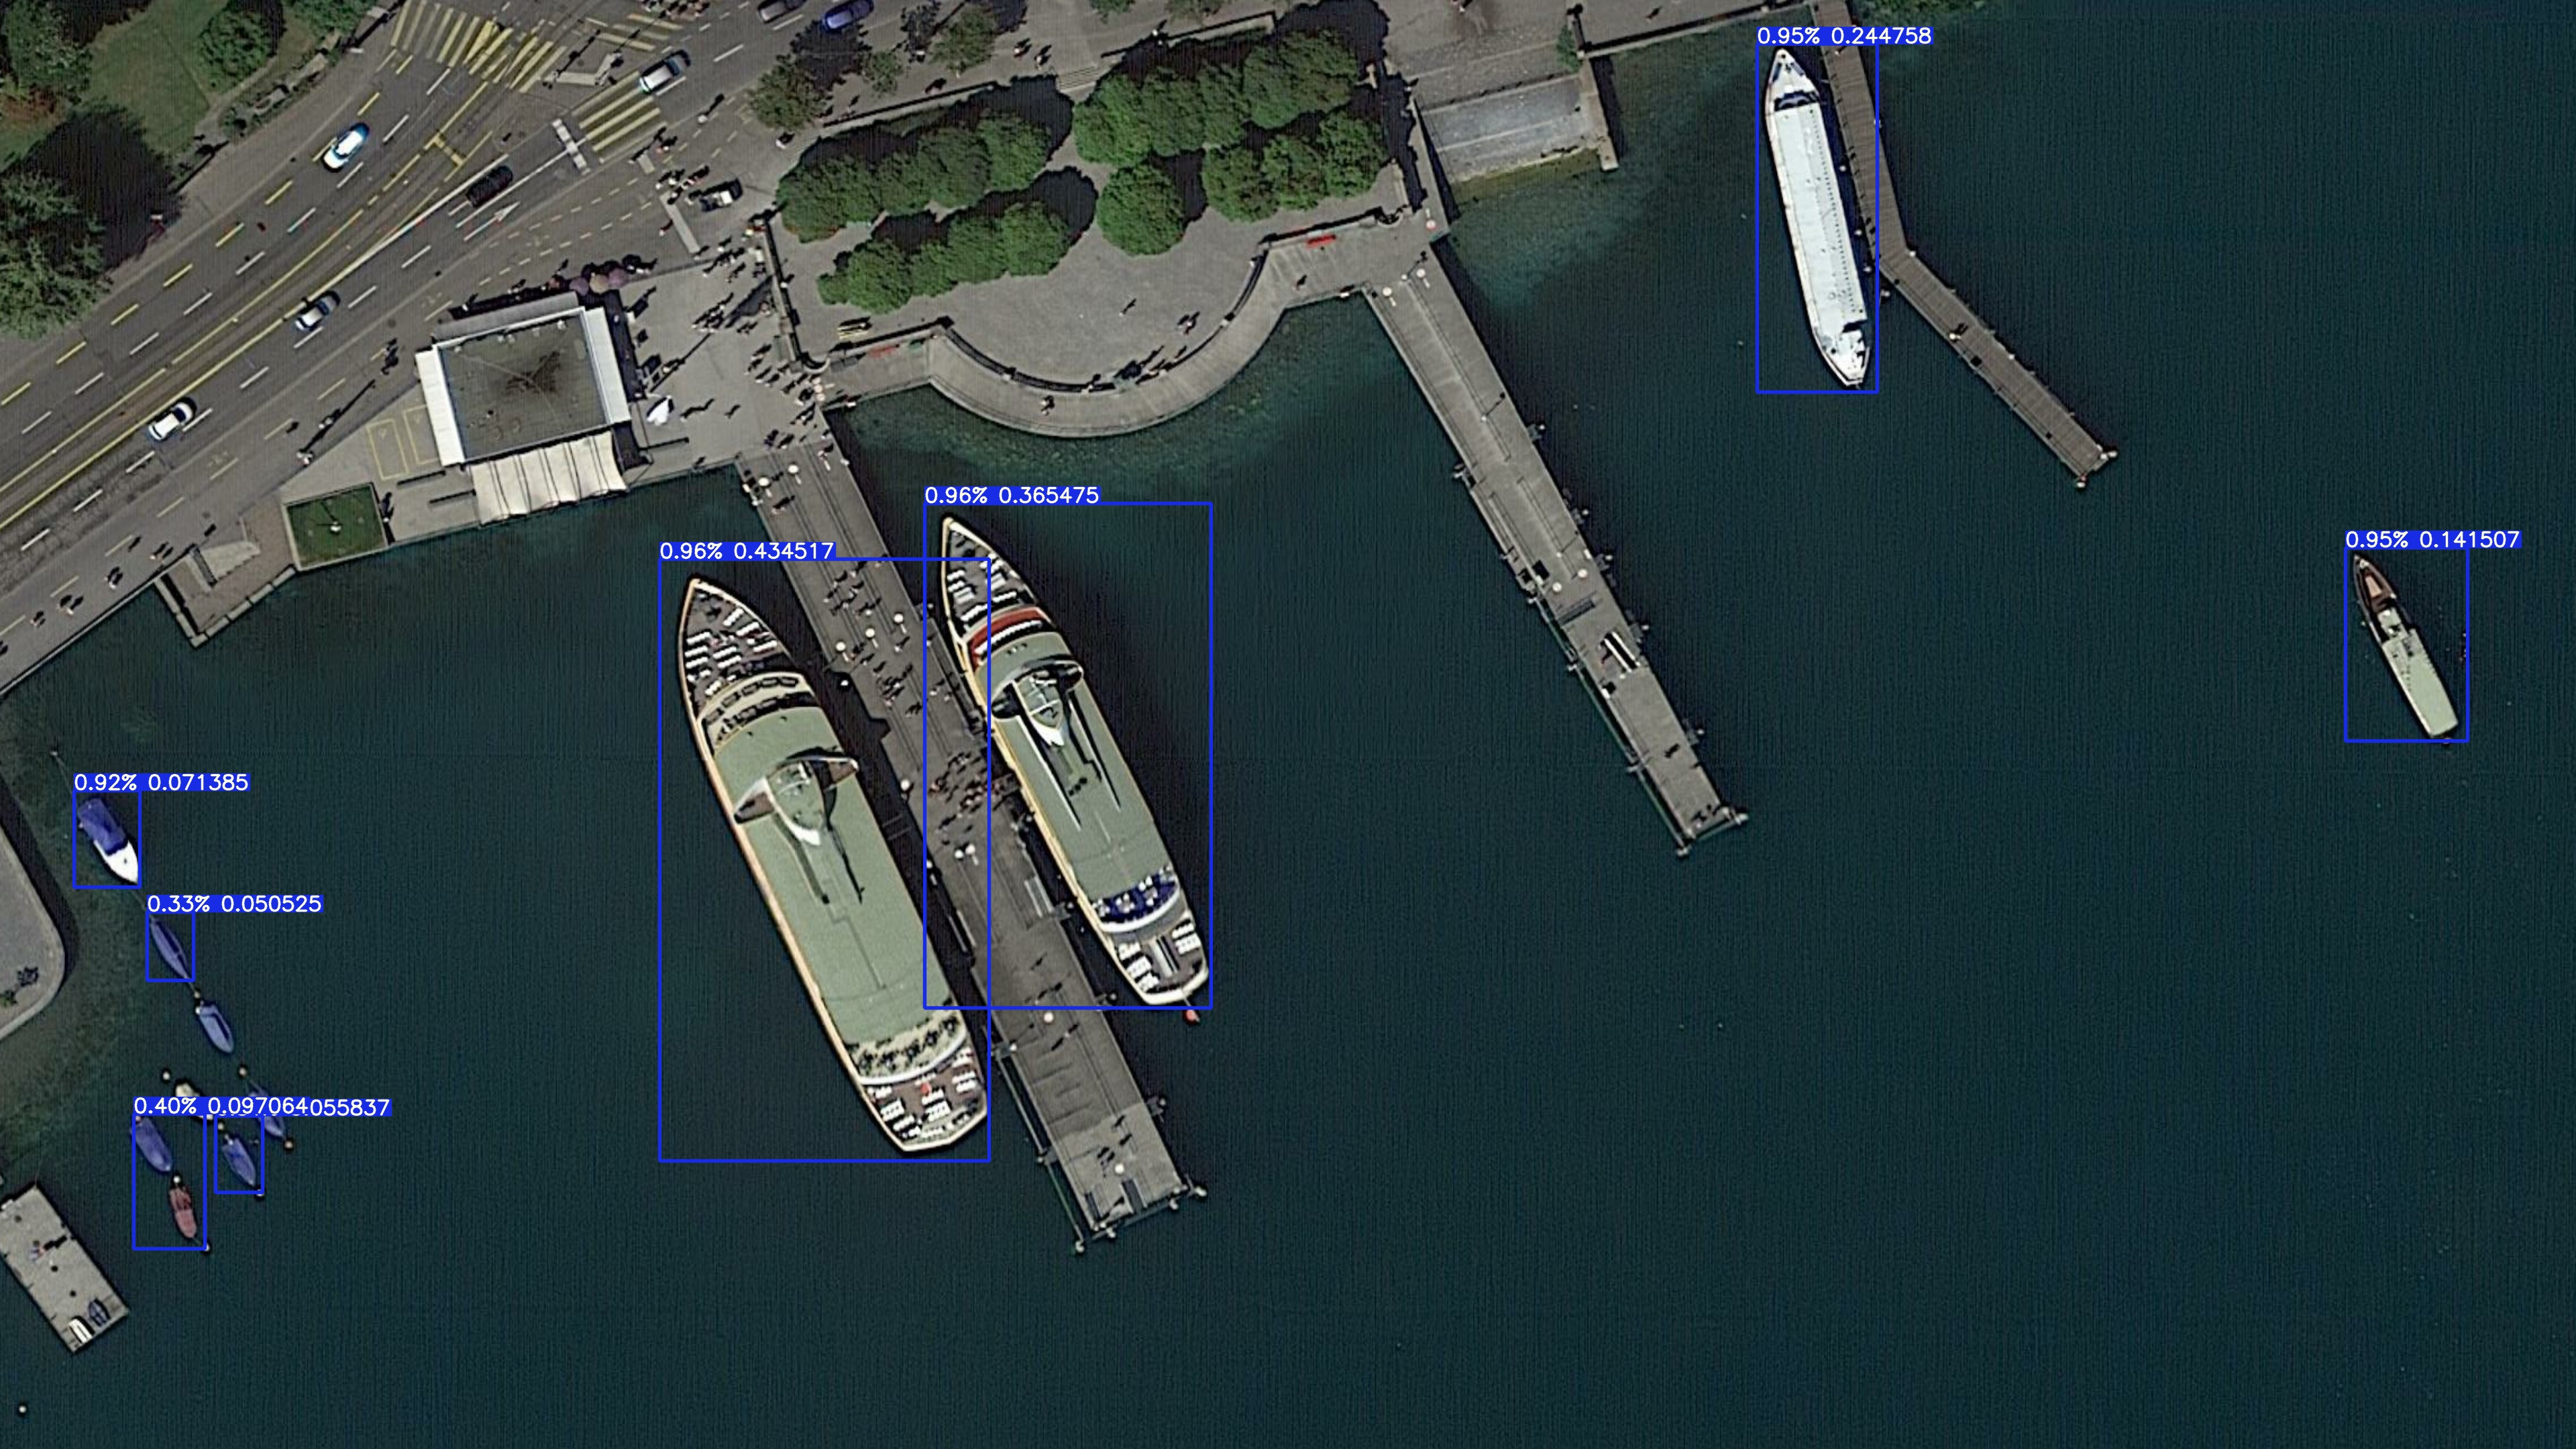
\includegraphics[width=\columnwidth]{img/zurich.jpeg}
    \caption{An image from Google Earth Pro for Zurich Lake on 16 Aug 2018 when eye alt is 200 meters.}
    \label{fig:zurich}
\end{figure}

Based on the above rules, the eye altitude was finally 200 meters. For this study it was used a satellite image of Zurich Lake, Switzerland, on 16th August 2018 as the standard image for defining the scale (Figure~\ref{fig:zurich}). Compared with other regions, the satellite image of Zurich Lake complies with the rules and it is a suitable candidate as the standard for measuring as a standard for measuring the length of small boats.

After measurement, the vessel in Figure~\ref{fig:zurich} had a YOLO length of 0.43 is 55.17 meters. Then, with an eye altitude of 200 meters, the ratio of the real length to the YOLO length is approximately 127. Finally, after several verifications, this ratio is within the margin of error and can be used as a scaling ratio. Moreover, having the same ratio and eye altitude is not enough. The resolution of each image needs to be the same so measurements are standardized. For this purpose, all datasets involved in the detection will maintain a resolution of 3840x2160 pixels which is the highest standard resolution in Google Earth.

In a certain sense, large vessels (e.g. cargo ships or warships) and small vessels (e.g. small boats for domestic use for recreation and fishing) are distinguished when creating the dataset for the area. However, due to the scaling, the eye altitude of the image is only 200 meters. Therefore, some large vessels, such as general cargo ships, do not even appear fully in an image, hence they are not considered in the statistical results of this work. On the other hand, some of the larger vessels, slightly shorter in length, are identified correctly by the algorithm and counted as part of the number of large vessels in the area. A Python script was then designed to count the number of small and large boats between regions.

After distinguishing between large and small boats, it is necessary to distinguish between small recreational boats for domestic use. For this work it was decided to start with two main categories, recreational boats and fishing boats without roof. To distinguish between them the model used the detected deck color of the the small boat. If the deck color was predominantly white then it was assigned as a recreational boat while any other mix of color will be assigned as a fishing both. It is recognized that this is a broad and simplistic classification method but it is an effective one to test the categorization power of the model. Each of the detected boats (i.e. the objects within the four coordinate anchor box) were analyzed whether the color was white or mainly white to then assign it to each category. As a final step the model performed the category counting for each image where a Python script was designed to count the small white boats.
